\chapter{System Description}\label{chap:systemDescribtion}

\section{Sensors}

\todo{describe the sensors}

\subsection{Magnetometer}

The orbit of the satellite is predictable, the satellite's location can be described as a function of time. Earth's magnetic field can also be quite accurately modeled. This means that by using magnetorquers, the orientation of the satellite can be approximated by comparing the magnetic field model at the satellite's current location and the direction of the magnetic field measured by the magnetometer. To address the noise in the measurement, including the noise arising from inside the satellite, Kalman or particle filtering, along with sensor fusion can be used, however this is outside of the scope of the thesis.

\subsection{Sun Tracking}

Sun trackers can be much easier to develop than star trackers. It measures the sun's orientation in relation to the satellite frame. By using it alongside other sensors, higher accuracy attitude estimation can be achieved, however when Earth is obstructing the sun rays, it is unable to provide attitude data, thus it is not sufficient to only use a sun tracking sensor.

\section{Actuators}
 
\subsection{Reaction Wheels}

One method of controlling a spacecraft's attitude is by using either reaction or momentum wheels attached to the spacecraft's body. By controlling the wheel's angular velocity using a motor, the amount of angular momentum stored in the wheel can be controlled. If there are no external forces involved, the sum of angular momentum in the system made up by the spacecraft's body and the reaction wheels is constant. This means that by increasing the angular velocity of the wheels, the satellite body's angular momentum can be reduced. This angular momentum transfer can be used to control the attitude of the satellite. If the goal is to change the angular momentum of the whole satellite, actuators that have external interaction should be used, such as magnetorquers or solar sails.

The difference between momentum and reaction wheels is that the nominal angular velocity of momentum wheels is high in order to store angular momentum, and in the case of reaction wheels, low. Many momentum wheels still turn at an angular velocity larger than zero in order to avoid static friction in the bearings. Reaction wheels usually make up only a small fraction of a satellite's weight. They rely on being able to run at high speeds, making their angular momentum significant. The small weight ratio makes precise controlling easier.


%One design consideration for reaction wheels is maximizing moment of inertia for unit weight. This is done by distributing most of the material near the outskirts of the wheel. There is a trade-off between having most of the mass at the outskirts and durability at high angular velocities. 


Reaction wheels have an angular velocity limitation. This means that if a reaction wheel reaches its maximum angular velocity, it can no longer generate a torque on the satellite's body in one direction. In this scenario the system's controllability decreases, thus it should be avoided. An angular momentum unloading strategy should be designed to avoid it. Instead of returning the angular momentum to the satellite's body, unloading the angular momentum through other methods is preferred. Magnetorquers can be used for such purposes.

Moving parts are usually prone to failures. Reaction wheels are expected to run at high angular velocities, which wears down the lubrication and the bearings. Reaction wheels equipped with active magnetic bearings are in development \cite{MagneticReactWheel}. These can eliminate friction from the system and by controlling the bearing, can even reduce micro-vibrations, increasing the durability of the system. AAUSAT-II itself however uses mechanical wheel bearings.

\subsection{Reaction Wheel Configuration}

angular acceleration demand \cite{reactionWheelConfigThesis} 

gps orientation, Earth station

Tetrahedron configuration can output twice as much force along an axis as one wheel can produce along its own axis.

\subsubsection{Transformation Between Body \& Reaction Wheel Space}

The main attitude controller sends torque demands to the actuators. The torque demand distributed to the reaction wheels have to be converted to torques parallel to reaction wheel axes, in order for the motor controllers to function. Transformation from reaction wheel space to body frame is quite intuitive. Knowing the orientation of each motor axis and the corresponding motor torque 
, the torque in body frame can be derived according to equation \ref{eq:motorTrans1} - \ref{transmatrix}. The matrix for tetrahedron configuration is given by \cite{reactionWheelConfigThesis}.

\begin{equation}
\label{eq:motorTrans1}
\vec{N_{rw}} = \underline{A}_{DC} \vec{N_{DC}} = \begin{bmatrix}
\vec{Axis^{DC}_{1}}       & \vec{Axis^{DC}_{2}}   & \vec{Axis^{DC}_{3}}   & \vec{Axis^{DC}_{4}} 
\end{bmatrix} \vec{N_{DC}}
\end{equation}

\begin{equation}
\underline{A}_{DC} \vec{N_{DC}}  = 
\begin{bmatrix}
\cos(19.47)       & -\cos(19.47) \cos(60)  &  -\cos(19.47) \cos(60)  & 0 \\
0       & \cos(19.47) \cos(30)  &  -\cos(19.47) \cos(30)  & 0 \\
-\sin(19.47)       & -\sin(19.47)   &  -\sin(19.47)   & 1
\end{bmatrix} \vec{N_{DC}}
\label{transmatrix}
\end{equation}

where $\vec{N_{rw}}$ is the reaction wheel torque in body frame, $\vec{N_{DC}}$ is the vector containing the reaction wheel DC motor torques parallel to their axes, $\vec{Axis^{DC}_{i}}$ are the reaction wheel motor orientation in body frame, $\underline{A}_{DC}$ is the transformation matrix between axis oriented reaction wheel torque and torques in 3 dimensional body frame.


\nomenclature[S]{$\vec{N_{rw}}$}{Reaction wheel torque in body frame }
\nomenclature[S]{$\vec{N_{DC}}$}{$4\times1$ vector containing the reaction wheel motor motor torques parallel to their axes }
\nomenclature[S]{$\underline{A}_{DC}$}{Transformation matrix between axis oriented reaction wheel torque and torques in 3 dimensional body frame }

Since $\underline{A}_{DC} $ is a $ 4 \times 3 $ matrix, a pseudo inverse has to be used when reordering the equation, as presented in equation \ref{eq:motorTrans}. 

\begin{equation}
\label{eq:motorTrans}
\vec{N_{DC}} =  \underline{A}_{DC} ^\dagger \vec{N_{rw}}   =  \underline{A}_{DC}^T  (\underline{A}_{DC} \underline{A}_{DC} ^T)^{-1} \vec{N_{DC}}
\end{equation}


%\begin{equation}
%h_{rot} = A\left[ h_1, h_2, h_3, h_4 \right]^T
%\end{equation}

In case there's a demand to adjust the torque distribution between the wheels, an extra vector can be included, as shown in equation \ref{eq:TorqueDistrib}
\cite[equation 18.41-42]{SADC}. If k is set to 0, the norm of wheel torques are minimized.

\begin{equation}
\label{eq:TorqueDistrib}
 \vec{N_{DC}} = \underline{A}^\dagger_{DC} \vec{N_{rw}}  + k\left[1,-1,-1,1\right]^T
\end{equation}


\subsubsection{Reconfiguration}

Fault isolation for the redundant reaction wheel configuration can be done by detecting which is the reaction wheel where the fault occurred and shutting it off and redistributing the torques to the rest of the reaction wheels. This reconfiguration can be represented by swapping the corresponding faulty columns to zero vectors. For example, if a fault occurs in the 3rd reaction wheel, the transformation matrix becomes $\underline{A}_{DC,f3}$, as presented in equation \ref{eq:ReactFault}.

\begin{equation}
\label{eq:ReactFault}
\underline{A}_{DC,f3} = \begin{bmatrix}
\vec{Axis^{DC}_{1}}       & \vec{Axis^{DC}_{2}}   & \vec{0}   & \vec{Axis^{DC}_{4}} 
\end{bmatrix} 
\end{equation}

\nomenclature[S]{$\underline{A}_{DC,fi}$}{Transformation matrix between axis oriented reaction wheel torque and torques in 3 dimensional body frame in case of faulty $i$th reaction wheel}

The pseudo inverse is calculated in the same manner as presented in equation \ref{eq:motorTrans}, as shown in equation \ref{eq:motorTransFault}. 

\begin{equation}
\label{eq:motorTransFault}
\underline{A}_{DC,f3}^\dagger   = \underline{A}_{DC,f3}^T  (\underline{A}_{DC,f3} \underline{A}_{DC,f3}^T)^{-1}
\end{equation}


\chapter{Actuators modelling and control}\label{chap: modeling}
 \textit{This chapter will describe the chosen reaction wheels and BLDC motors along with the electrical and mechanical modelling of the motors.} 
%
\section{Reaction wheels}
%
%Since the focus of the current thesis is not on the design of reaction wheels, only few constraints are  taken into account for the selection of the wheels, such as the weight and the inertia. In order to minimize the total weight of the satellite, the weight of each wheel, is not overcome the %weight of each motor. 

The satellite should be capable of tracking an Earth station in order to be able to downlink data effectively. Tracking a ship requires similar control capability, since the velocity of the wheel is practically zero compared to the velocity of the satellite. Directing the satellite to the nadir continuously only requires keeping a satellite angular velocity equal to the orbit's angular velocity.
Pointing the antennas to the Earth station requires torque from the actuators, the torque demand can be calculated based on the angular acceleration demand for Earth station tracking.
%


 The wheel moment of inertia is \cite{flywheel_design_thesis} $I_{w} = 2.456 [gcm^2]$ and the weight is $m_{w} = 4.201 [g] $ compared to the motor weight $m_{motor} =8 [g] $ and the motor shaft moment of inertia $I_{motor} = 0.0249 [gcm^2]$. The characteristics of the selected motor can be found in appendix \ref{chap: B}. The maximal speed of the motor is $\omega_{max}= 20000[rpm]$ and thus the maximum angular momentum that the system wheel-motor can provide can be found as    
%
%\nomenclature[S]{\textbf{$J_{wheel}$}}{Reaction wheel inertia}
%\nomenclature[S]{\textbf{$J_{motor}$}}{Motor inertia}
%\nomenclature[S]{\textbf{$m_{motor}$}}{Weight of the motor}
%\nomenclature[S]{\textbf{$m_{wheel}$}}{Weight of the reaction wheel}
\begin{flalign*}
	h_{max} = {J_{wheel}} {\omega_{max}} 
\end{flalign*}
%\nomenclature[S]{\textbf{$h_{max}$}}{Maximum angular momentum of the wheel-motor system}
%0.000114450   5.1438e-04
which is found to be $5.1438\cdot10^{-4} [Kgm^2/s]$ for each wheel.	
%
%
For three axis stabilization, three wheels each orthogonal to the principal axis, are efficient but in case of one actuator failure it jeopardizes controllability of the satellite. To avoid this, redundancy is desired, requiring four wheels in tilted positions. The configuration of the wheels is chosen to be in tetrahedron shape giving rise to more reliable and robust system. The tetrahedron configuration will be discussed in section \ref{ref:reactConfig}.  
\subsection{BLDC motor model}
\label{sec:motors}

In order to make the system more reliable, brush-less DC motors are chosen as actuators. BLDC motors are lighter compared to brushed with the same power output and do not causing sparking thus can be used in operations that demand long life and reliability.
%
%\nomenclature[A]{\textbf{BLDC}}{Brushless Direct Current }
Each motor consists of an electrical part and a mechanical part. The electrical part of the motor can be modeled using Kirchhoff's Voltage Law as
%
\begin{flalign}
 V_{a} -V_{R}-V_{L} -V_{e} = 0
\label{Kirchhoff1}
\end{flalign}
%
%\nomenclature[S]{\textbf{$V_{a}$}}{Voltage source }
%\nomenclature[S]{\textbf{$V_{R}$}}{Voltage drop across the resistance }
%\nomenclature[S]{\textbf{$V_{L}$}}{Voltage drop across the inductance }
where $V_{a}$ is the voltage source, $V_{R}$ is the voltage drop across the resistance, $V_{L}$ is the voltage drop across the inductance and $V_{e}$ is the back emf. Equation \ref{Kirchhoff1} can be re written as 
%
%\nomenclature[S]{\textbf{$V_{e}$}}{Back electromotive force- emf }
\begin{flalign}
	V_{a}= R_{a}i + L_{a}\dfrac{di}{dt}+ k_{e}\omega
	\label{Kirchhoff244}
\end{flalign}
%
%\nomenclature[S]{\textbf{$R_{a}$}}{Armature resistance}
%\nomenclature[S]{\textbf{$L_{a}$}}{Armature inductance}
%\nomenclature[S]{\textbf{$k_{e}$}}{Back emf coefficient}
 where $R_{a}$ [Ohm] is the armature resistance, $L_{a}$ [H] is the armature inductance and $k_{e}$ is the back emf coefficient as it can be seen in the \figref{fig:electromech} .   
%

\begin{figure}[H]
	\begin{minipage}[b]{0.49\linewidth}
		\centering
		\begin{figure}[H]
			\centering
			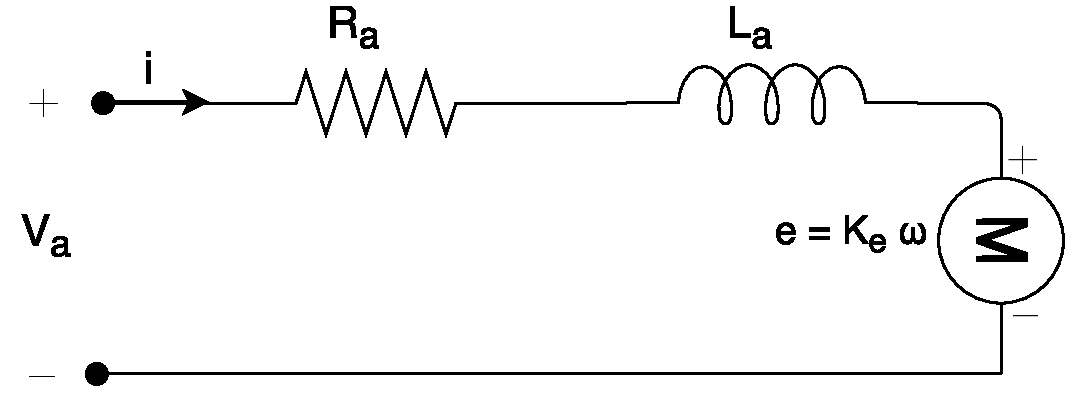
\includegraphics[width=1\linewidth]{figures/BLDC_el.pdf}
			%\caption{ Electrical and mechanical part of the motor }
		%	\label{fig:electromech}
		\end{figure}
	\end{minipage}\hfill
	\begin{minipage}[b]{0.49\linewidth}
		\centering
		\begin{figure}[H]
			\centering
			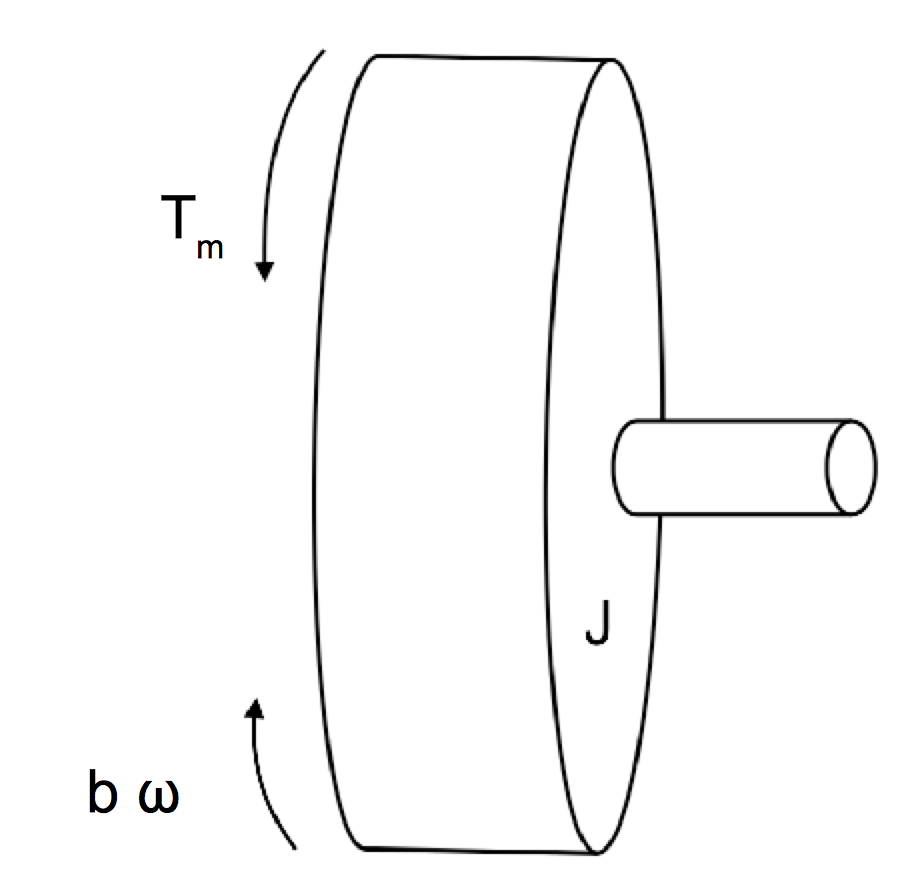
\includegraphics[width=0.55\linewidth]{figures/flywheel_1}
			%\caption{Mechanical part of the motor}
			%\label{fig:distancecontrol4}
		\end{figure}
	\end{minipage}
	\caption{ Electrical and mechanical part of the motor }
	\label{fig:electromech}
\end{figure}

%
The mechanical part of the motor can be modelled as 
%
\begin{flalign}
 k_{t}i  =J\dfrac{d\omega}{dt} + b\omega
	\label{mechpart66}
\end{flalign}
%
%\nomenclature[S]{\textbf{$k_{t}$}}{Motor torque coefficient}
%\nomenclature[S]{\textbf{$b$}}{Viscous friction coefficient}
where $J$ is the rotor moment of inertia, $k_{t}$ [Nm/A] is the motor torque coefficient and $b$ [Nm s/rad] is the viscous friction coefficient. %Assuming the current will not increase rapidly in order not to harm the equipment, and moreover the electrical time constant $\tau_{e}=\dfrac{L}{R}$ is much smaller than the mechanical time constant $\tau_{m}=\dfrac{J}{b}$, the effect of the inductance can be neglected and the
 Equation \ref{mechpart66} can be solved for $i$ and  replaced in \ref{Kirchhoff244}\cite{permanent_magnet}     
%
\begin{flalign}
	i  =\dfrac{J}{k_{t}}\dfrac{d\omega}{dt} + \dfrac{b}{k_{t}}\omega
	\label{mechpart2}
\end{flalign}
%
\begin{flalign}
 V_{a} = \dfrac{LJ}{k_{t}}\dfrac{d^{2}\omega}{dt^{2}}+\dfrac{RJ+Lb}{k_{t}}\dfrac{d\omega}{dt} +\dfrac{Rbk_{e}}{k_{t}}\omega 
	\label{mechpart333}
\end{flalign}
%
by Laplace transformed \ref{mechpart333}, the second order transfer function from $V_{a}$ to $ \omega $ can be written as 
%
\begin{flalign}
	\dfrac{\omega(s)}{V_{a}(s)}= \dfrac{k_{t}}{LJs^{2}+(RJ+Lb)s+(Rb+k_{e}k_{t})}
	\label{tf}
\end{flalign}
%= \dfrac{k_{t}}{LJs^{2}+(RJ+Lb)s+Rb+k_{e}k_{t}}
%\label{tf}
following \cite{permanent_magnet} the electrical time constant $\tau_{e}$ and mechanical time constant $\tau_{m}$ can be written respectively $\tau_{e} = \frac{LJ}{RJ+Lb}$ and $\tau_{m} = \frac{RJ+LB}{RB+k_{e}k_{t}}$, the values for the two time constants are found to be $\tau_{e} = 1.2709\cdot10^{-10}$[s] and $\tau_{m} = 8.4102\cdot10^{-4}$[s] thus since the $\tau_{e}$ is very small compared to $\tau_{m}$, the effect of inductance can be neglected thus the transfer function from $V_{a}$ to $ \omega $ is reduced to a first order transfer function as 
%
\begin{flalign}
\dfrac{\omega(s)}{V_{a}(s)}= \dfrac{k_{t}}{R(Js+b)+k_{e}k_{t}}
\label{tf2}
\end{flalign}
%
the block diagram of the system can be seen in figure \ref{fig:blockdi} along with PI velocity controller which will be discussed in the next section.
%
%\nomenclature[S]{\textbf{$\tau_{e}$}}{Electrical time constant}
%\nomenclature[S]{\textbf{$\tau_{m}$}}{Mechanical time constant}
\begin{figure}[H]
	\centering
	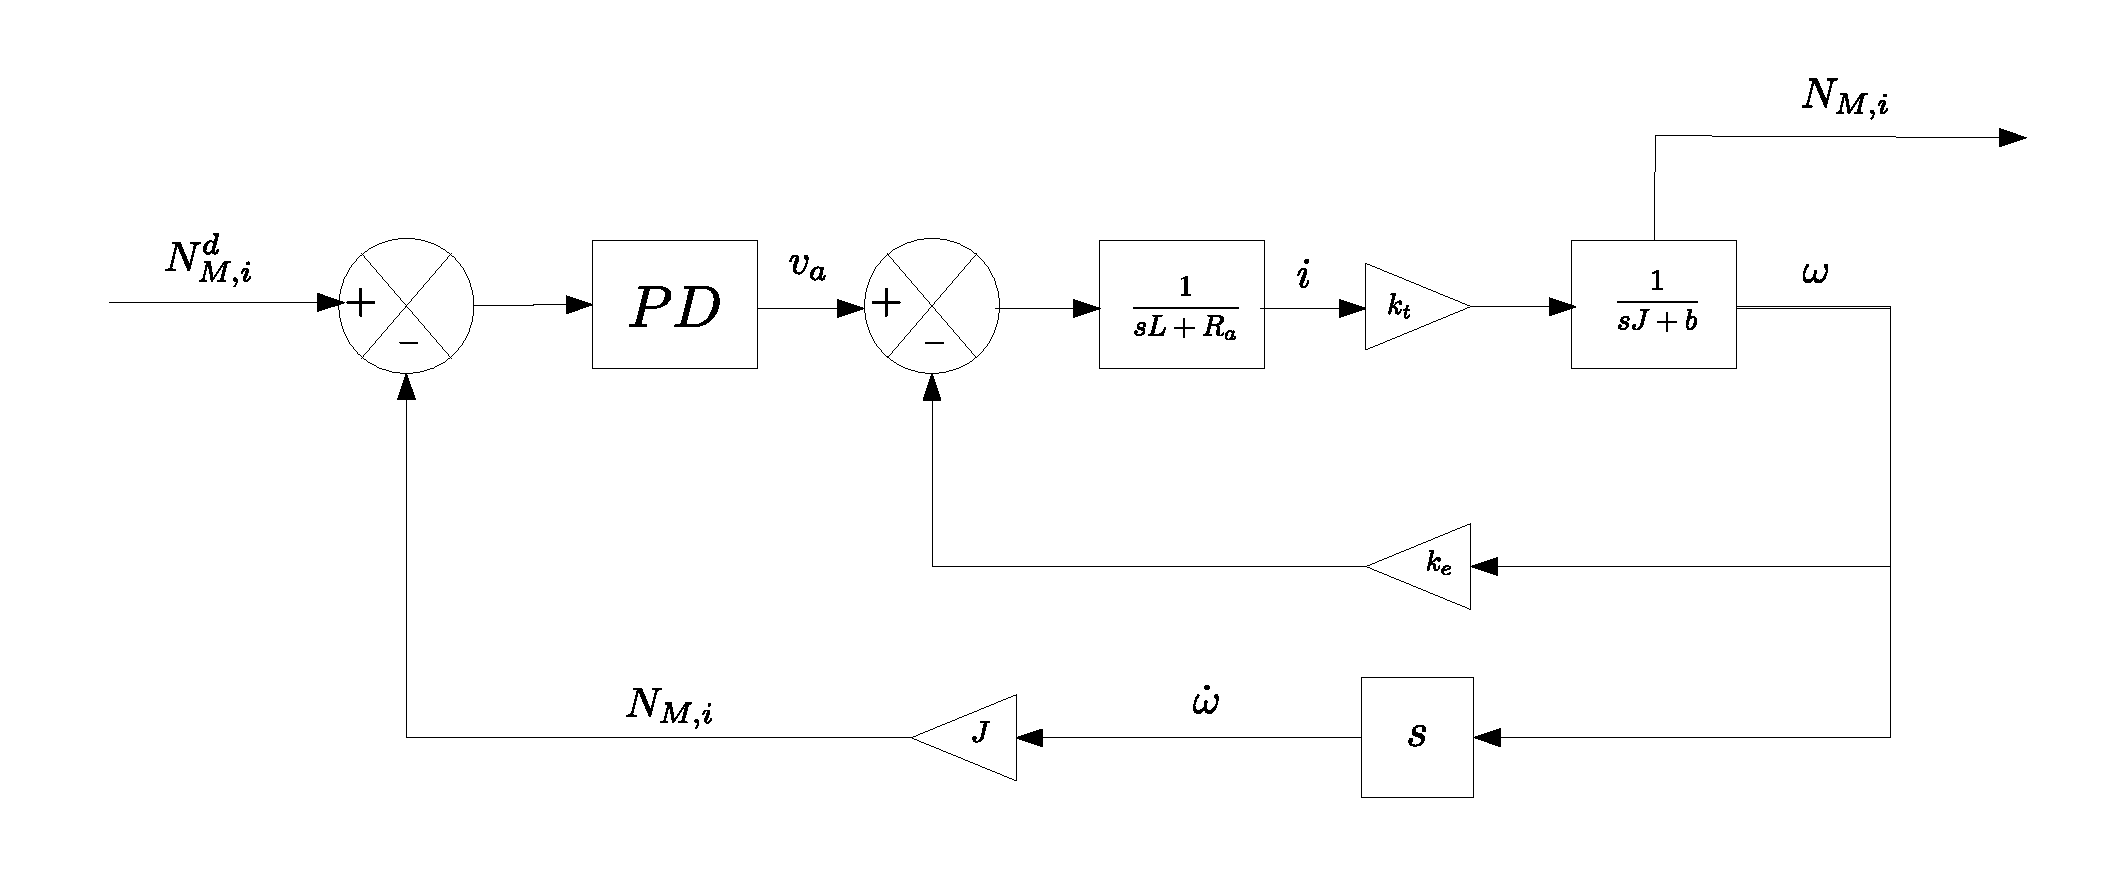
\includegraphics[width=1\linewidth]{figures/omegaControl}
	\caption{Angular velocity controlled DC motor}
	\label{fig:blockdi}
\end{figure}
%

% 
\chapter{Motor control}

\subsection*{ Angular velocity control}

In previous work, two controllers a linear and a non-linear(SMC), have been designed requiring a torque that has to be produced from the motors-wheel system. This torque demand is used to give the desired angular velocity reference for the wheels and thus the torque that will be fed back to the satellite as seen in the \cite{block diagram}. The output torque from the linear and non-linear controllers has three elements which has to be transformed in the tetrahedron configuration using the matrix \eqref{transmatrix}.  A \textit{PID} controller has been designed to control the angular velocity of the motor as seen in the \figref{fig:blockdi222}:
\begin{figure}[H]
	\centering
	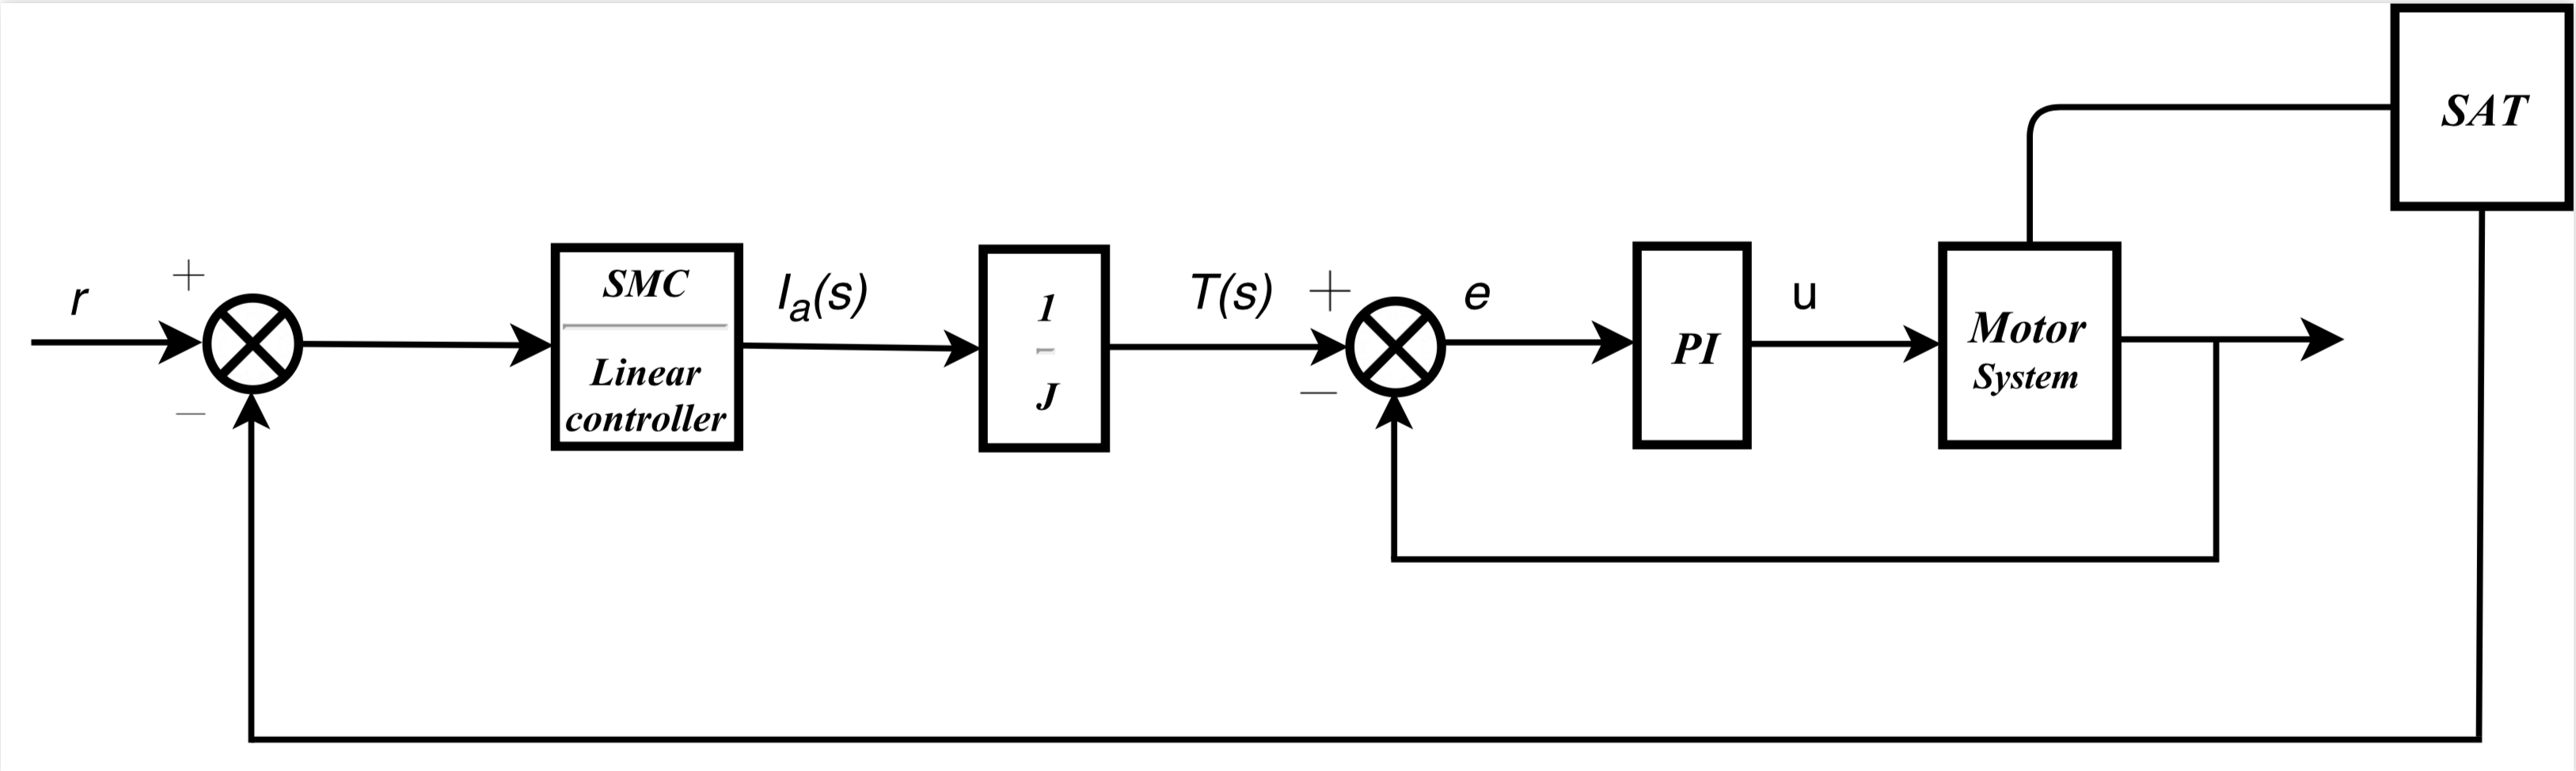
\includegraphics[width=1.0\linewidth]{figures/block_diagram_2}
	\caption{Block diagram of the motor control with PID controller}
	\label{fig:blockdi222}
\end{figure}  
%
The PI controller gains are chosen based on the open loop system response using the Ziegler-Nichols method \cite{PID_tuning} and by trial and error in order to achieve faster closed loop response and asymptotically stable system. The gains are chosen to be:   
%
\begin{flalign*}
	k_{p} = 3.4 \\ k_{i} = 0.9
\end{flalign*}

\todo{make figure bigger}
The root locus of one motor with PI controller is seen in the \figref{fig:rlocus33}
%
\begin{figure}[H]
	\centering
	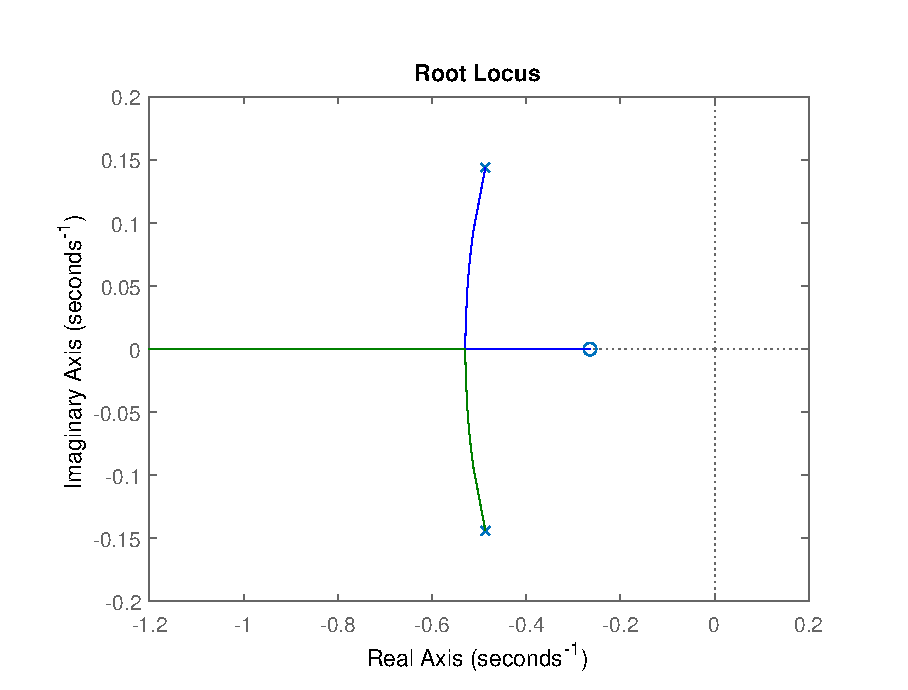
\includegraphics[width=0.7\linewidth]{figures/pid_rootlocus}
	\caption{Root locus of one motor with PI controller}
	\label{fig:rlocus33}
\end{figure}
%
The closed loop system gives complex eigenvalues and fast response and is stable for a wide range of the adjustable parameters. 
%

%

\subsection{Torque Control}

The main attitude controller sends a torque demand to the actuators, which is then distributed between the actuators. Each of the reaction wheels get their own individual torque demand signals. Two methods have been implemented for tracking this torque demand. One is by transforming the torque to angular velocity demand, which the motor has to track, the other is directly controlling for actuator error.

\begin{figure}[h!]
	\centering 
	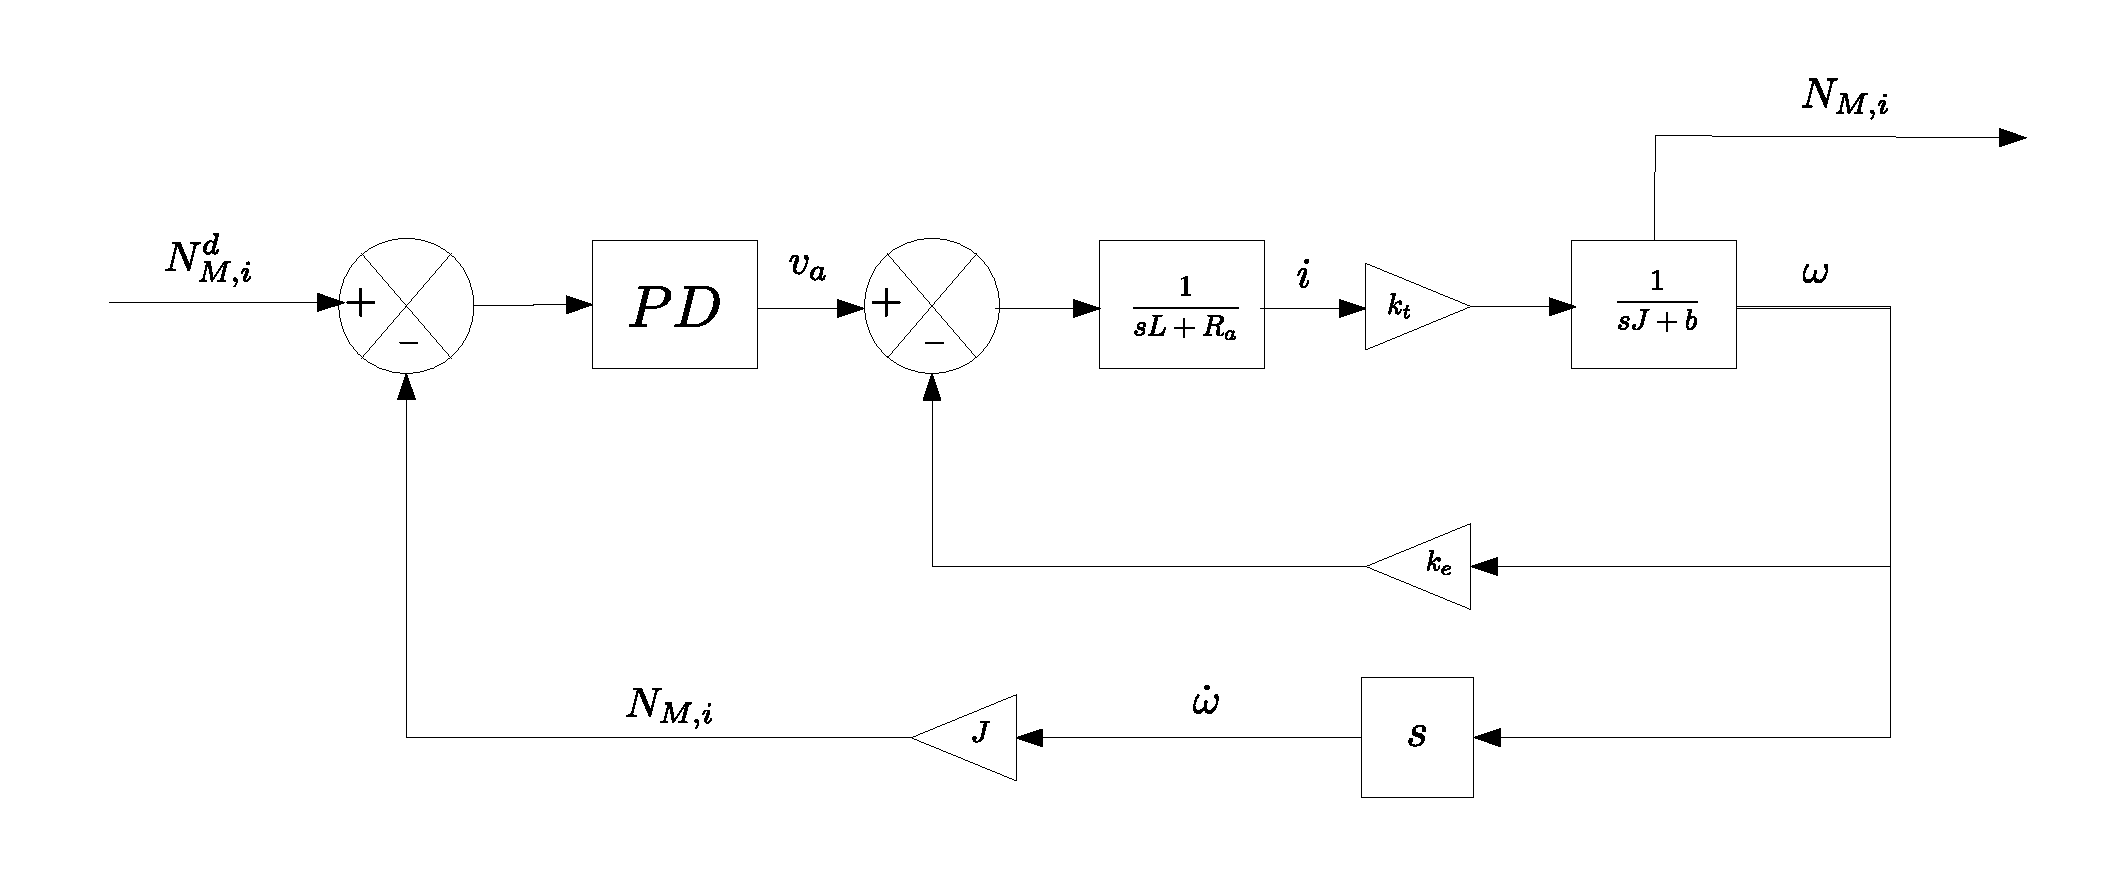
\includegraphics[width=170mm]{figures/torqueControl.pdf}	
	\caption{Torque control scheme.}
	\label{label{fig:frames}}
\end{figure}

As shown on Figure XY , the torque controller controls the torque error signal using a PD controller. Since the torque has a $ 10^{-5} Nm$ magnitude, while the voltage has $ 10^1 V$, numerically the PD gains are quite large. The control signal is the input voltage for the DC motor. The subsystem is second order, including an integrator for current and one for angular velocity.

\section*{Magnetorquer model}
\nomenclature[Sncoil]{$n_{coil}$}{The number of windings of the coil}
\nomenclature[SIcoil]{$I_{coil}$}{The electric current flowing through the coil}
\nomenclature[SAcoil]{$\vec A_{coil}$}{The vector perpendicular to the cross-sectional area of the magnetorquer}
\nomenclature[Sm]{$\vec m_{mt}$}{The magnetic dipole moment}

Since the primary actuators for the satellite are chosen to be reaction wheels, four magnetorquer will be used for desaturation of the reaction wheels.  

Having a solenoid onboard of the satellite, referred as a magnetorquer through which the current could be controlled and hence the dipole moment.

The interaction of the dipole with the magnetic field of the Earth will result in a torque that will be perpendicular to the magnetic field vector according to the following equation \cite{SADC}:
\begin{flalign}
   \vec N_{mt} = \vec m_{mt} \times \vec B
	\label{eq:NT}
\end{flalign} 
where $\vec N$ is the torque produce by the magnetorquer and will be the torque that will influence the satellite dynamics, $\vec B$ is the vector of the magnetic field of the Earth and $\vec m_{mt} $ is the magnetic dipole moment generated by the magnetorquer.

The magnetic moment $\vec m_{mt}$ is given by \cite{MagMom}:
\begin{flalign}
	\vec m_{mt} = n_{coil} \ I_{coil} \ \vec A_{coil}
	\label{eq:mm}
\end{flalign} 
where $n_{coil}$ is the windings of the coil, $I_{coil}$ is the electric current on the coil and $\vec A_{coil}$ is the vector perpendicular to the cross-sectional area of the magnetorquer.

Using \ref{eq:NT} and \ref{eq:mm} and taking the magnitude, the applied torque on the satellite is \cite{SJ}:
\begin{flalign}
	\vec N_{mt} = n_{coil} \ \rvert I_{coil}\rvert \ \rvert \vec A_{coil}\rvert \ |\vec B| \sin (\theta)
	\label{eq:ft}
\end{flalign} 
where $\sin (\theta)$ is the angle between the plane $A_{coil}$ and the magnetic field vector $\vec B$.

Furthermore, the resistance of the magnetorqer which is a function of the temperature of the coil given as an input, can be computed as
\begin{flalign}
R_{mt} = \dfrac{nC  \rho_{mt} }{A_{wire}} = \dfrac{nC \rho_0(1+\alpha_0(T_{mt} - T_0))}{A_{wire}}
\label{eq:rt}
\end{flalign} 
where \\
$R_{mt}$ is the resistance of the magnetorquer \\
$n$ is the number of windings \\ 
$C$ is the wire circumference  \\
$A_{wire}$ is the wire cross-sectional area  \\
$\rho_0$ is the resistivity of copper  \\
$\alpha_0$ is the coefficient of resistivity temperature   \\
$T_{mt}$ is the temperature given as an input   \\
$T_0$ is the resistivity base temperature  

Using the computed resistance the current is found by dividing the voltage by the resistance of the magnetorquer. Next, in order to find the magnetic moment $m$, the current is multiplied by the number of windings and the area of the wire. For finding the torque that acts on the satellite, the magnetic moment is multiplied by the coil normal and a cross-product is used between this multiplication and the magnetic field of the Earth.

In order to find what voltage to output for having a certain amount of torque, a gain between voltage and magnetic moment is found. For the coil model, the control signal is the voltage. Therefore, translating the magnetic moment demand to voltage is found as follows:
\begin{flalign}
\frac{\vec m_{mt}}{v} = \frac{n_{coil} \vec A_{coil} \vec I_{coil}}{R_{mt}} \mathcal {K}
	\label{eq:gain}
\end{flalign} 
\begin{flalign}
 \mathcal{K} = \frac{\vec m_{mt} R_{mt} }{ n_{coil}  \vec A_{coil} \vec I_{coil} v}
	\label{eq:gainn}
\end{flalign} 
where \\
$v$ is the voltage \\
$\mathcal {K}$ is the gain

The voltage can be found using the following transfer function:
\begin{flalign}
	\frac{I_{coil}}{v} = \frac{1}{R_{mt}}
	\label{eq:voltage}
\end{flalign} 

where the voltage is found to be $1.25 V$

Given a current $I$ going through a coil, the interest is to find the magnetic field $B$ at a certain point located distance $r$ from the coil. Finding an estimate of the magnetic field at any point will give the possibility to change the location of the magnetometers around. For computing the magnetic field in the center of a rectangular coil, the law of Biot-Savart is used \cite{SJ}:
\begin{flalign}
	d\vec B = \frac{\mu_0 I}{4 \pi}  \frac{d \vec s \times \hat{\vec r}}{r^2}
	\label{eq:BS}
\end{flalign} 
where \\
$\vec B$ is the magnetic field \\
$\mu_0$ is a constant called permeability of free space and is equal with $4\pi \times 10^{-7}  \ Tm/A$ \\
$I$ is the current \\
$d \vec s $ is a length element in the direction of current \\
$\hat{\vec r}$ is the direction from $d \vec s$ to a particular position \\
$r$ is the distance from $d \vec s$ to a particular position

The magnetic field $B$ at any point is directly proportional to the current $I$ that is crossing the coil. The magnetic field generated by the current from equation \ref{eq:BS} is just a small length element $d \vec s$ of the coil. For finding the total magnetic field, all small elements need to be summed up and for this the magnetic field $B$ have to be evaluated by integrating equation \ref{eq:BS}.

The design of the magnetorquer is described in appendix \ref{chap:F}.

